\begin{enumerate}
  \item 非空集合 $X, Y$
  \item 法则 $f$
  \item $X$ 中的每个元素 $x$,在法则 $f$ 下,能从 $Y$ 中找到\textbf{唯一}的值 $y$ ,即: $y = f(x)$
\end{enumerate}

\begin{equation}
f:X \to Y
\end{equation}

\paragraph{}
x与y关系:一对一、多对一


\begin{figure}[H]
\centering
  %------- 第1行 -------
  \begin{subfigure}[t]{0.4\linewidth}
    \centering
      % x 与 y 关系,一对一
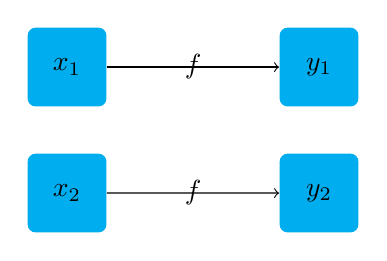
\begin{tikzpicture}[scale=0.8]
  \node [fill=cyan,minimum size=1cm,rounded corners=.1cm]   (x1) at (0,0)    {$x_1$};
  \node [fill=cyan,minimum size=1cm,rounded corners=.1cm]   (x2) at (0,-2)   {$x_2$};
  \node [fill=cyan,minimum size=1cm,rounded corners=.1cm]   (y1) at (4,0)   {$y_1$};
  \node [fill=cyan,minimum size=1cm,rounded corners=.1cm]   (y2) at (4,-2)   {$y_2$};

  \draw [->] (x1) -- (y1) node[midway] {$f$};
  \draw [->] (x2) -- (y2) node[midway] {$f$};
\end{tikzpicture}

      \caption{一对一}
  \end{subfigure}
  \begin{subfigure}[t]{0.4\linewidth}
    \centering
      % x 与 y 关系,多对一
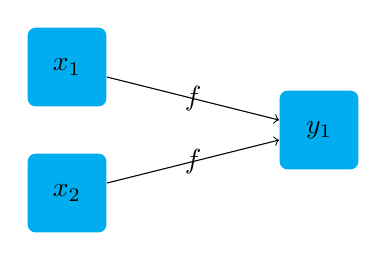
\begin{tikzpicture}[scale=0.8]
  \node [fill=cyan,minimum size=1cm,rounded corners=.1cm]   (x1) at (0,0)    {$x_1$};
  \node [fill=cyan,minimum size=1cm,rounded corners=.1cm]   (x2) at (0,-2)   {$x_2$};
  \node [fill=cyan,minimum size=1cm,rounded corners=.1cm]   (y1) at (4,-1)   {$y_1$};

  \draw [->] (x1) -- (y1) node[midway] {$f$};
  \draw [->] (x2) -- (y1) node[midway] {$f$};
\end{tikzpicture}

      \caption{多对一}
  \end{subfigure}
  \caption{x 与 y 关系}
\end{figure}

\paragraph{}
\textbf{概念}

\begin{enumerate}
  \item 定义域(Domain):$D_f = X$
  \item 值域(Range):$R_f = Y = f(x)$
\end{enumerate}

\begin{enumerate}
  \item 满射:$Y$ 中任意一个元素 $y$,都是 $X$ 中某一元素的像
  \item 单射:$X$ 中任意两个元素 $x_1 \neq  x_2$,它们的像不一样,$f(x_1) \neq  f(x_2)$
  \item 双射(一一映射):满足单射和满射条件
\end{enumerate}

\subsection{逆映射}

\begin{enumerate}
  \item $f$ 是 $X$ 到 $Y$ 的单射
  \item 则逆映射 $f^{-1} = g$,值域 $R_f$ 到 $X$ 的映射,即 $g(y) = x$
\end{enumerate}

\begin{equation}
g:R_f \to X
\end{equation}

\subsection{复合映射}

\begin{enumerate}
  \item 设有两个映射 $g:X \to Y_1$,$f:Y_2 \to Z$
  \item $Y_1 \subset Y_2$
  \item 则 $X$ 到 $Z$ 的映射,记作:$f \circ g$
\end{enumerate}

\begin{gather}
f \circ g: X \to Z \\
(f \circ g)(x) = f[g(x)], x \in X
\end{gather}
